\section{Theorie}
\label{sec:Theorie}

Atome Kerne die ein unausgeglichenes Verhältnis zwischen Protonen und Neutronen aufweisen, zerfallen nach einem gewissen Zeitraum.
Dieser hängt vom Atom ab.
Die Zeit, bis zu der das instabile Atom zerfällt kann mit der Halbwertszeit $T$ beschrieben werden.
Diese gibt an wie viel Zeit vergeht bis die Hälfte des Stoffes $N_0$ zerfallen ist.
Die Zeit welche vergeht bis nur noch die Hälfte des Stoffes vorhanden ist kann dabei durch 
\begin{equation*}
    \frac{1}{2}N_0 = N_0 \text{e}^{-\lambda t}
\end{equation*}
berechnet werden.
$\lambda$ ist hier die Zerfallskonstante des Isotops.
Daraus folgt die Halbwertszeit $T$ mit 
\begin{equation}
    T = \frac{\ln{2}}{\lambda}.
    \label{eqn:Halbwertszeit}
\end{equation}
Die Halbwertszeit verschiedener Stoffe variiert sehr stark, in diesem Versuch sollen nur Methoden besprochen werden, 
um Halbwertszeiten im Bereich von Sekunden und Minuten zu bestimmen.
\\\\
Da diese Stoffe schnell zerfallen werden sie erst kurz vor der Messung hergestellt.
Hierfür werden die stabilen Atome mit Neutronen aus einer Neutronenquelle beschossen.
Durch das zusätzliche Neutron befinden sich die Atome nun im instabilem Zustand und zerfallen schließlich.
Der Zerfall findet dabei, in diesem Versuch immer in Form eines $\beta$- oder $\gamma$-Zerfalls statt.
Die Neutronen sollten dabei eine möglichst geringe Energie haben.
Denn die Resonanzabsorption des Atoms findet genau dann statt wenn das Neutronen, genau die Energie aufweist, die der Differenz zweier Energieniveaus des Zwischenkerns entspricht.
Diese ist entsprechend klein, weswegen die Neutronen erst gebremst werden müssen bevor sie auf das Atom geschossen werden.
Wie diese thermischen Neutronen erzeugt werden, wird im Abschnitt \ref{sec:Durchführung} ausführlich erklärt.
\\\\
Da es äußerst Schwierig ist die Stoffmenge $N$ zuverlässig im Verlauf des Zerfalls zu bestimmen wird eine Methode genutzt, welche sich durch das Messen der abgegebene Strahlung realiesieren lässt.
Dafür müssen nur die in einem Zeitintervall $\Delta t$ zerfallenen Kerne $N_{\Delta t}(t)$ gemessen werden.
Mithilfe der Gleichung 
\begin{equation}
    \ln{N_{\Delta t}(t)}=\ln N_0 (1-e^{-\lambda \Delta t}) -\lambda t
    \label{eqn:labmda}
\end{equation}
lässt sich durch eine lineare Ausgleichsrechnung anschließend $\lambda$ bestimmen, welches zur Bestimmung der Halbwertszeit benötigt wird.
\\\\
Wenn nun aber das Isotop in zwei verschiedene Isotope zerfällt überlagern sich die Strahlungsmuster beider Isotope miteinander.
Eine schmatische Darstellung, einer Zerfallskurve, zweier Isotope mit unterschiedlichen Zerfallskonstanten $\lambda$ ist in Abbildung \ref{fig:zerfall2} zu finden.
Wie zu sehen ist erschwert dies die Ermittlung der beiden Halbwertszeiten.
In diesem Fall muss zunächst die Halbwertszeit des langlebigen Isotops bestimmt werden.
\\\\
Dies geschieht indem nur die Werte betrachtet werden, die nach dem Zeitpunkt $t*$ aufgenommen wurden.
Diese Werte werden für eine lineare Ausgleichsrechnung genutzt, wodurch eine Annäherung des Zerfalls des langsam zerfallenden Isotops gemacht wird.
Die ermittelte Gleichung wird genutzt um, die Zerfallskonstante $\lambda_1$ des schnell zerfallenden Isotops zu berechnen.
Zusätzlich können mithilfe einer Extrapolation, die Werte des langsam zerfallenden Isotops von den aufgenommenen Messwerten abgezogen werden.
Mit den so berechneten Werten wird eine weitere Ausgleichsrechnung angefertigt mit der die Zerfallskonstante $\lambda_2$ des schnell zerfallenden Isotops bestimmt wird.
Nun kann mit den Zerfallskonstanten die Halbwertszeit der beiden Isotope berechnet werden.

\begin{figure}
    \centering
    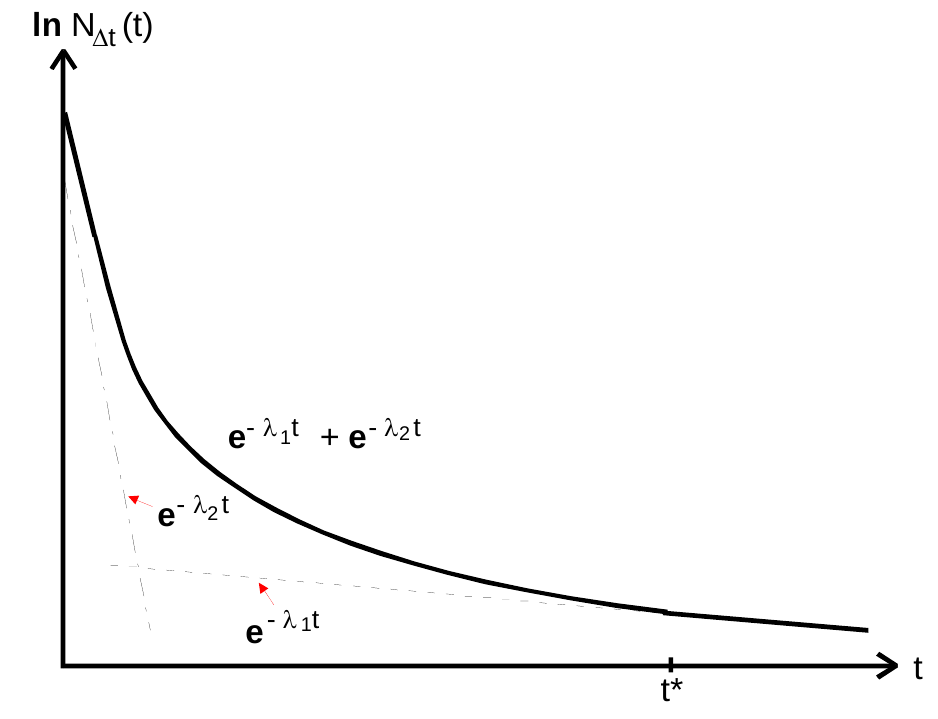
\includegraphics[width=0.6\textwidth]{content/data/zerfall.png}
    \caption{Der Zerfall zwei verschiedener Isotope mit unterschiedlichen Halbwertszeiten. Entnommen aus Quelle \cite{anleitung}.}
    \label{fig:zerfall2}
\end{figure}